\documentclass[11pt]{exam}

\usepackage{amsmath}
\usepackage{graphicx}
\usepackage{geometry}
\usepackage{etoolbox}
\BeforeBeginEnvironment{choices}{\par\nopagebreak\minipage{\linewidth}}
\AfterEndEnvironment{choices}{\endminipage}
\geometry{
a4paper,
total={185mm,257mm},
left=10mm,
top=25mm,
bottom=10mm
}

\begin{document}
\setlength{\voffset}{-0.5in}
\setlength{\headsep}{5pt}

\fbox{\fbox{\parbox{8cm}{\centering
\vspace{2mm}
Testat - Versuch E - Diffusion und Osmose 
\vspace{2mm}
}}}
\hspace{2mm}
\makebox[0.25\textwidth]{Name:\enspace\hrulefill} \hspace{5mm}
\makebox[0.2\textwidth]{Datum:\enspace\hrulefill}
\vspace{4mm}

\begin{questions}

\question Die Leitfähigkeit von 20 ml Salzlösung wird zu 5,0 \( \frac{\mu S}{cm} \) bestimmt. Welches Volumen an destilliertem Wasser muss zugeführt werden, um eine Leitfähigkeit von 10,0 \( \frac{\mu S}{cm} \) zu messen?

\begin{choices}
	\choice 0 ml
	\choice 20 ml
	\choice 10 ml
	\choice keine Antwort richtig
	\choice 30 ml
\end{choices}

\vspace{3mm}\question Welcher Verlauf ist im ersten Versuchsteil für die Messung der Leitfähigkeit in Abhängigkeit der Salzkonzentration zu erwarten? 

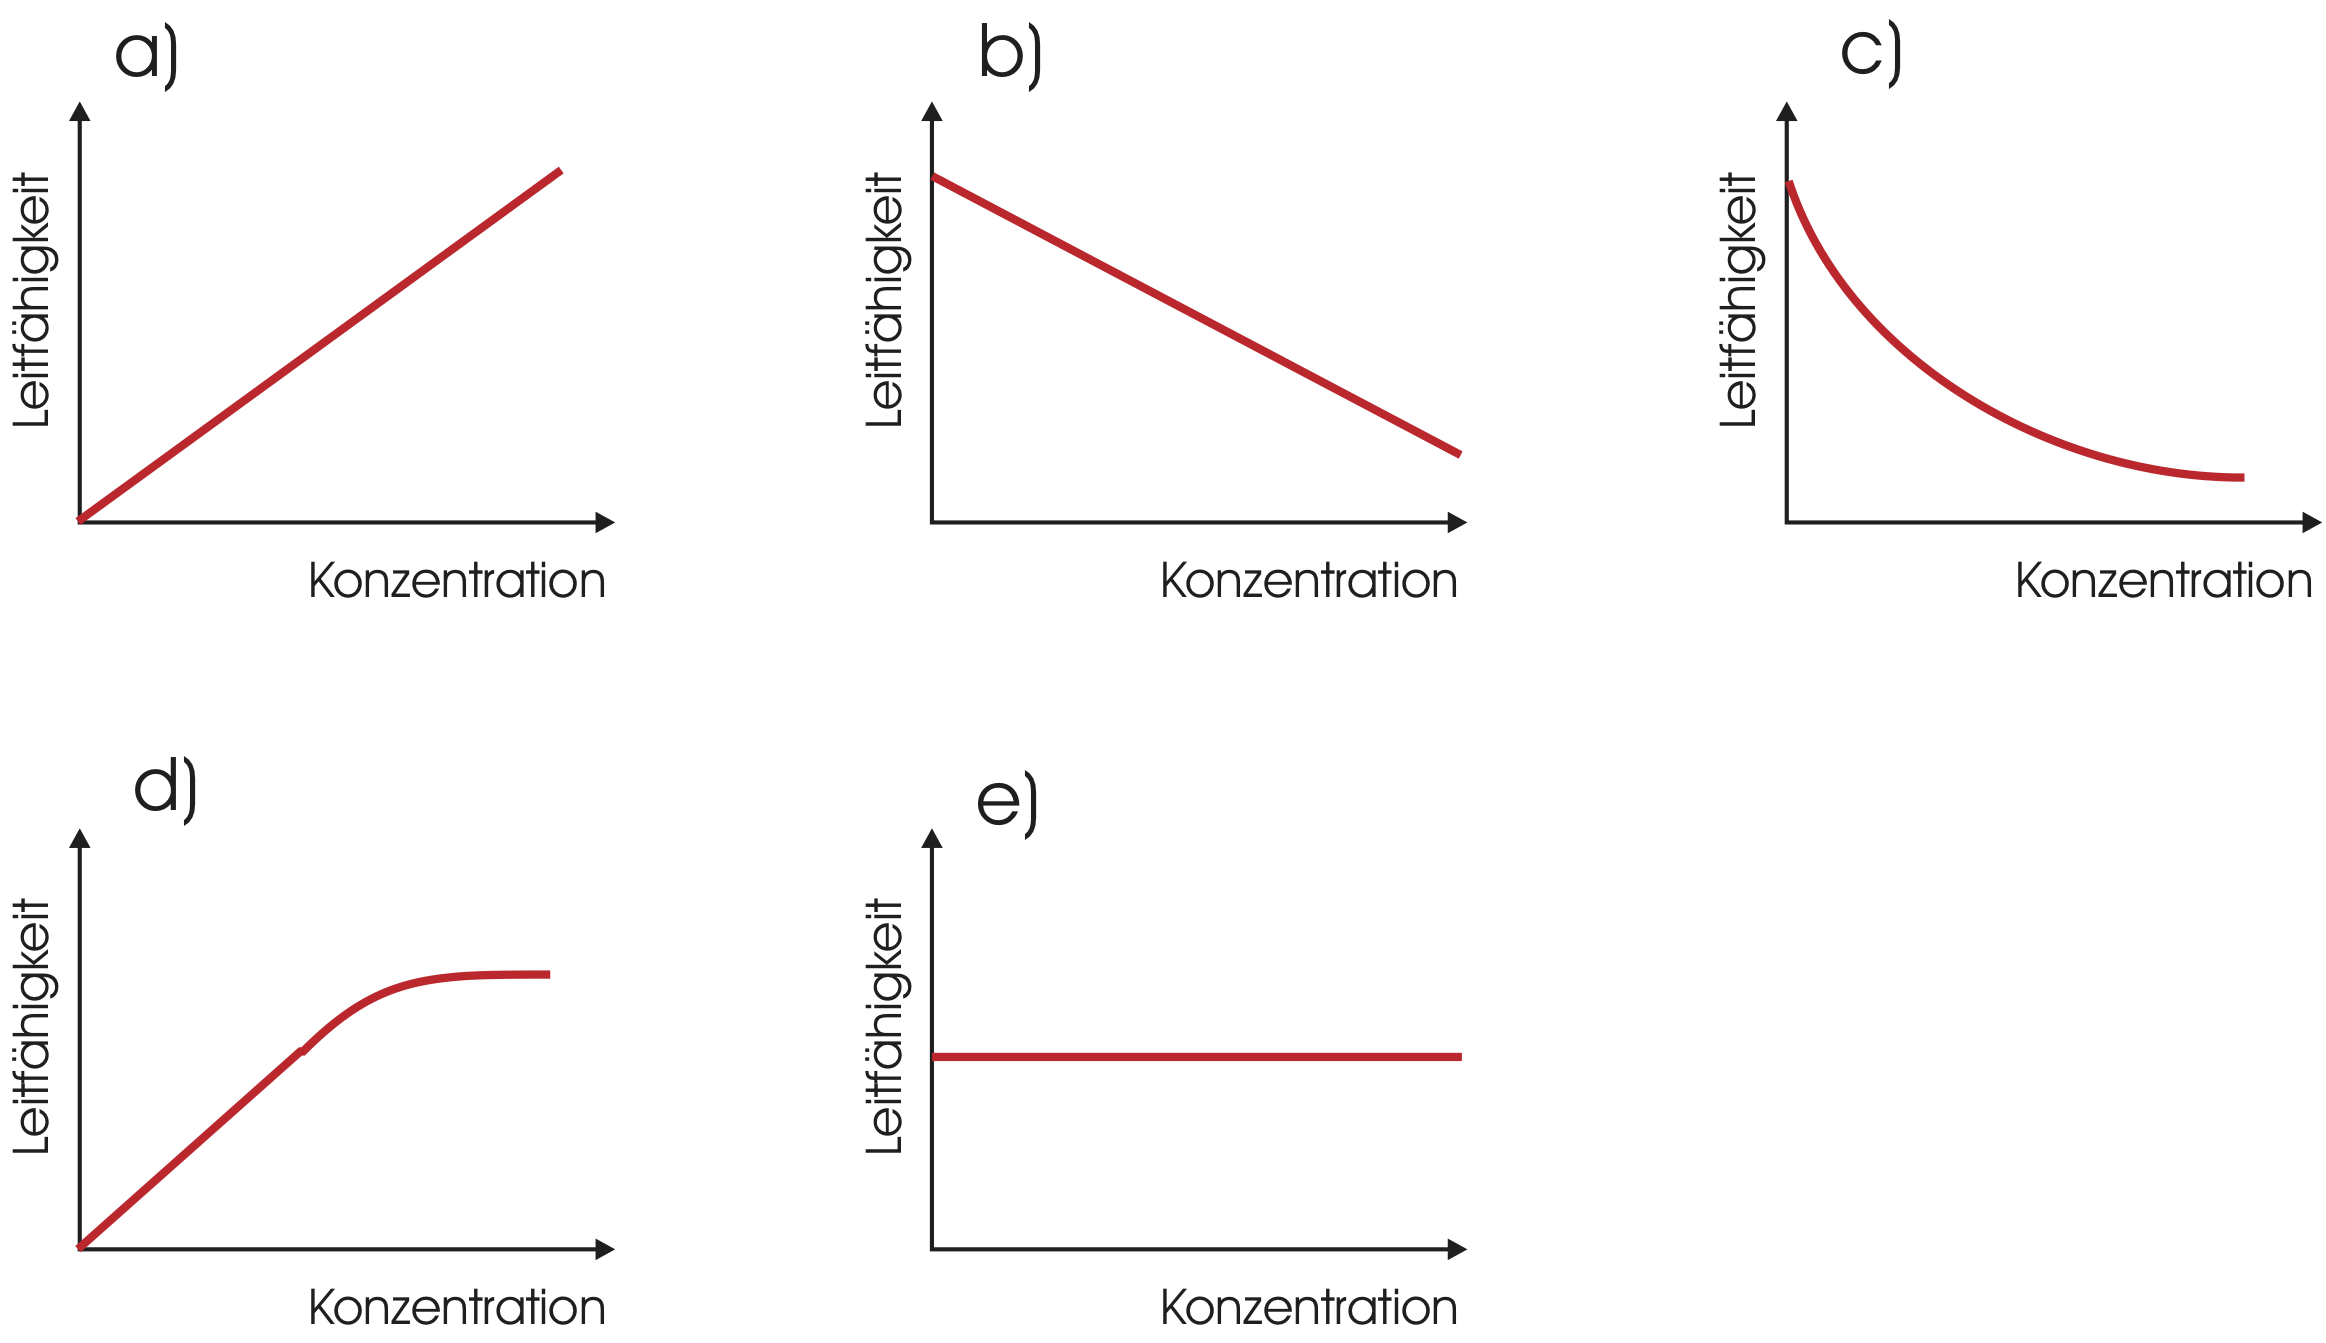
\includegraphics[width=0.4\textwidth]{images/Leitfaehigkeit.png}

\begin{choices}
	\choice c)
	\choice d)
	\choice e)
	\choice b)
	\choice a)
\end{choices}

\vspace{3mm}\question Von welchen Parametern ist der Diffusionsfluss durch ein Membran abhängig?A) TemperaturB) Ladung der TeilchenC) Größe der diffundierenden TeilchenD) Größe der Membranporen

\begin{choices}
	\choice keine Antwort
	\choice alle Antworten
	\choice A und B
	\choice A, C und D
	\choice B und C
\end{choices}

\vspace{3mm}\question Wo spielt Diffusion in der Natur keine Rolle?

\begin{choices}
	\choice Gasaustausch bei der Lungenatmung
	\choice Bildung des Zellpotentials
	\choice Bewegung von Amöben
	\choice Bildung von Ödemen
	\choice Filtration in der Niere
\end{choices}

\vspace{3mm}\question Von welchen Größen hängt der osmotische Druck eines gelösten Stoffes ab?

\begin{choices}
	\choice Dichte und Diffusionskoeffizient des Stoffes
	\choice Gyrationsradius und Konzentration des Stoffes
	\choice Nur vom Van't-Hoff-Faktor des Stoffes
	\choice Konzentration des Stoffes und Temperatur
	\choice Molare Masse und Ladung des Stoffes
\end{choices}

\vspace{3mm}\end{questions}

\end{document}
